\section{Experimental Protocol}
\subsection{Synthetic mechanism study}
Predictive input follows \(x\sim\mathcal N(0,I_2)\), independently of context \(c\sim\mathcal N(\mu_d,0.45^2I_2)\). Domain \(d\) labels by \(\mathbf{1}[v_d^\top x\geq0]\), then flips each label independently with probability 0.05. The best population accuracy with the correct rule is approximately 95\%.

Benign shifts use contexts \((0,0),(5,0),(0,5)\) and one rule \((1,0.6)\), in order A,B,C,A,B,C. Conflicting shifts keep those contexts and order but use rules \((1,0.6),(-1,-0.6),(0.6,-1)\). Mixed recurrence uses four contexts \((0,0),(5,0),(0,5),(0,10)\), with A/B sharing the first rule and C/D its opposite, in order A,B,C,D,A,B,C,D. Hidden reversal uses identical contexts and opposite rules, in order A,B,A,B,A,B. A fixed input-only router cannot determine which opposite concept generated an observation; their balanced expected accuracy is 50\%.

Each segment has 24 windows of 64 examples. The first 24 windows are a fixed warm-up. Replay stores 256 observations, and each optimizer step draws 32 eligible examples. Each unique domain has 1,024 held-out examples per seed. Seeds 0--9 define ten matched streams, yielding 160 primary runs across four policies and four scenarios. The three earlier sensitivity configurations use persistence one or interference thresholds zero and 0.4, producing 480 additional configuration runs. They are exploratory analyses prompted by primary behavior; only corrected canonical runs are used.

\subsection{Real-image neural extension}
MNIST contains 60,000 training and 10,000 test images of handwritten digits \cite{mnist}. We preserve the official split and divide training positions further: 0--9999 are development-only, while 10000--59999 supply formal streams. Independent development trains on 6,000 images sampled from the first 8,000 and validates on positions 8000--9999. Its 89.8\% accuracy establishes a basic learnability check, not a final test result. Calibration uses unlabeled positions 0--1999 within the development partition.

For each formal seed, a permutation of the 50,000-image training pool supplies six disjoint chunks of 6,000. Every stream therefore contains 36,000 distinct source training images, 360 windows and no within-run image repetition. Domain recurrence uses new source images with the same transformation. Cross-seed training subsets can overlap; seeds are replications of a constructed task, not independent datasets.

Contrast uses A:\(x\), B:\(0.55x\), and C:\(0.55x+0.25\), preserving labels and order A,B,C,A,B,C. This tests shared semantic labels under intensity changes. It does not assert that the exact decision function is unchanged in pixel coordinates. Permutation uses identity and two fixed, seed-specific permutations of 784 pixel positions, with labels unchanged and the same recurrence order. Both networks and router receive only the transformed pixels.

Each domain is evaluated on all 10,000 official test images with its corresponding transformation. No test image or label enters calibration, replay or optimization. Test images are reused across domain transformations, policies, endpoints and seeds, so the resulting measurements are dependent. These short recurring streams differ from conventional published Permuted-MNIST protocols in data budget, sequence, architecture and access to task information.

Five matched seeds 0--4 compare Fixed, Novelty, Interference, Dual and Retained, giving 50 runs. Network initialization, training examples, transformations, test images and reservoir priorities are matched within each scenario/seed. The two-stream protocol was written before loading official test arrays. It was motivated by earlier synthetic results and is not an external preregistration. Learning rate, thresholds, lifetime and seeds were not selected using formal test accuracy.

\begin{table}[t]
\caption{Neural extension settings; differences from synthetic settings are explicit in the text.}
\label{tab:settings}\centering\small
\begin{tabular}{lr}\toprule Setting & Value\\\midrule
Network & 784--128--64--10\\
Trainable parameters per expert & 109,386\\
Examples per window / segment & 100 / 6,000\\
Optimizer steps / learning rate & 4 / 0.1\\
Replay capacity / batch & 512 / 64\\
Reference batch (maximum) & 64\\
Expert / prototype caps & 4 / 12\\
Trigger / gallery persistence & 3 / 3 windows\\
Cooldown / warm-up & 3 / 60 windows\\
Retained-evidence lifetime & 30 windows\\
Interference / novelty thresholds & 0.2 / 1.42039\\
Held-out images per domain & 10,000\\
Matched seeds & 5\\\bottomrule\end{tabular}
\end{table}

\begin{figure*}[t]\centering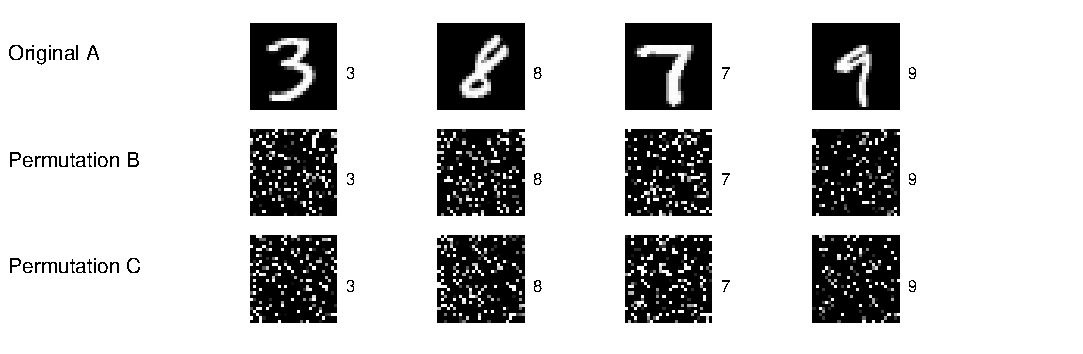
\includegraphics[width=\textwidth]{mnist_examples.pdf}
\caption{Actual MNIST training images under the seed-zero pixel transformations. Numbers beside images are original digit labels, retained in the initial permutation stream; the additional stress remaps them by domain. These examples are not generated images.}
\label{fig:mnist}\end{figure*}

\subsection{Additional conflict stress}
After the two-stream neural experiment started, we documented a separate exploratory stress. It retains the pixel permutations but changes domain labels to \((y+3d)\bmod10\), for \(d=0,1,2\). All other settings, images and seeds remain unchanged, adding 25 runs. This deliberately changes target meaning and is not ordinary digit recognition. Different permutations still supply information that can distinguish the domains, so one sufficiently expressive network can in principle fit all three mappings.

The stress is reported alongside every policy, with its post-start design status explicit. It is not an independent dataset confirmation, because it shares MNIST images and the same model family. No threshold or learning-rate search follows its test outcomes. A transformation that creates incompatible target mappings also need not create a sustained negative gradient streak in a flexible network; the logged score tests this assumption directly.

\subsection{Metrics and descriptive uncertainty}
After each segment, the evaluator tests all unique domains observed so far. Final accuracy is their unweighted mean, without increasing a domain's weight when it recurs:
\begin{equation}
A_T=D^{-1}\sum_{d=1}^D a_{T,d}.
\end{equation}
Forgetting uses endpoints after a domain first appears:
\begin{equation}
F_T=D^{-1}\sum_d\left(\max_{j\in J_d}a_{j,d}-a_{T,d}\right),
\end{equation}
where \(J_d\) includes the final endpoint. It is nonnegative but can miss within-segment failures. We also record experts, blocked requests, prototypes, gradient-sample appearances, retained-array bytes and CPU learner time. Allocated counts include unreachable experts; inference selects one network.

Tables give means and sample standard deviations. Matched seed differences use percentile bootstrap intervals: 5,000 resamples for synthetic and 10,000 for neural comparisons. They are descriptive, uncorrected for multiple comparisons and limited by ten or five independent seed pairs. The neural protocol specifies a one-percentage-point accuracy tolerance for a favorable descriptive accuracy--capacity comparison: the difference interval's lower endpoint must be above -1 point and mean allocation must decrease. This new criterion is not retroactively applied to synthetic results and is not a formal noninferiority proof.

\subsection{Implementation, checks and provenance}
Both studies use Python 3.12.14 and NumPy 2.3.5 on CPU. Neural matrix operations use one OpenBLAS thread. No PyTorch, GPU training, pretrained weights or downloaded learned representation is used. Raw MNIST archives are fetched from the mirror used by torchvision, checked against its four published MD5 values, and retained with SHA-256 provenance.

Nine synthetic checks cover gradients, historical isolation, test rejection, memory, budgets and routing assumptions. Eight neural checks additionally validate all three affine-layer gradients on a small model, parameter counts, clone independence, priority sampling, early allocation, disjoint source-image streams and a controlled delayed-conflict sequence. In that controlled sequence, retaining evidence permits a late expansion that the original conjunction misses. This verifies the implemented decision rule; it does not demonstrate a neural accuracy gain.

A previous synthetic bug overwrote old routing under early novel allocation. Corrected canonical runs preserve old anchors; archived pre-fix runs are excluded. The corrected source is shared across the four synthetic configurations. The neural source is separate and preserved exactly in both neural result directories.

The neural audit recomputes final accuracy and forgetting from raw endpoint records, checks matching hashes, source-index separation and caps, and reloads one checkpoint per policy/scenario. All fifteen reloaded models reproduce their stored final held-out accuracy. Checkpoints contain inference parameters and routing anchors, not the reservoir and RNG state required to resume optimization. Local code, protocols, manifests, raw logs and model files accompany this working project; no public repository is claimed. A real accessible repository link should replace local availability before a reproducibility-oriented public release.

